% <-- chapter -->
\chapter{Configurazione del server}
\label{ch:server}


% <-- section -->
\section{Overview della configurazione e prerequisiti}

In questa sezione andremo a installare e configurare OpenVPN server sulla VPS di OVHCloud.

Supponiamo di partire da una configurazione di base, che contiene solo il server openvpn ed un generico client, che supponiamo sia sotto un NAT.

Supponiamo inoltre che che l'ip pubblico del \it{server} sia \code{51.178.141.119}, si avra' quindi una configurazione come in figura \ref{fig:diag-simple_ips}.

\begin{figure}[h]

    \centering

    \begin{subfigure}{0.5\textwidth}
        \centering
        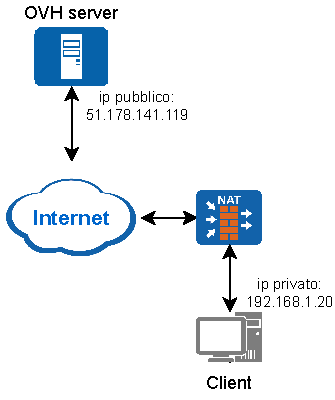
\includegraphics[height=1.2\linewidth]{immagini/diag-simple_ips}
        \caption{Configurazione di partenza per questo capitolo.}
        \label{fig:diag-simple_ips}
    \end{subfigure}%
    \hfill
    \begin{subfigure}{0.5\textwidth}
        \centering
        \includegraphics[height=1.2\linewidth]{immagini/diag-simple_ips_vpn}
        \caption{Configurazione virtuale da raggiungere.}
        \label{fig:diag-simple_ips_vpn}
    \end{subfigure}%
    \caption{Configurazione di partenza e di obbiettivo per questo capitolo. \cite{icons}}
\end{figure}

Per instaurare una comunicazione bidirezionale tra il server e il client, si dovra' configurare oppornunamente una rete vpn la cui configurazione e' rappresentata in figura \ref{fig:diag-simple_ips_vpn}.


I pacchetti necessari sono \code{openvpn} ed \code{easy-rsa}, che possono essere installati con:

\begin{bashcode}
$ sudo apt-get update
$ sudo apt-get install -y openvpn easy-rsa
\end{bashcode}

E' inoltre necessario avere un editor di testo, ad es. \code{nano} o \code{vim}


% <-- section -->
\section{Creazione della Public key infrastructure Certificate Authority (PKI CA)}

%TODO mettere intro su che diamine e' la pki https://datatracker.ietf.org/doc/html/rfc5280

La CA puo' essere configurata sulla stessa macchina dove e' stato installato opnevpn, ma cio' e' sconsigliato per motivi di sicurezza, supponiamo quindi di usare un secondo server chiamato \textit{server CA}

La utility \code{easy-rsa} mette a disposizione il comando \code{make-cadir}, che permette di creare una cartella pronta ad ospitare la Certificate Authority.

Andiamo quindi a crearla, nella home ad esempio:

\begin{bashcode}
$ mkdir ~/openvpn-ca
$ ln -s /usr/share/easy-rsa/* ~/openvpn-ca/
$ chmod 700 /home/ubuntu/openvpn-ca/
$ cd openvpn-ca/
$ ./easyrsa init-pki

init-pki complete; you may now create a CA or requests.
Your newly created PKI dir is: /home/ubuntu/openvpn-ca/pki

$ la
easyrsa  openssl-easyrsa.cnf  pki  vars.example  x509-types
\end{bashcode}

Ora si devono personalizzare le variabili \code{vars}, si puo' sia partire da un file vuoto oppure modificare \code{vars.example} per poi rinominarlo \code{vars}.
Andiamo quindi a creare un nuovo file vars:

\begin{bashcode}
$ vim vars
set_var EASYRSA_REQ_COUNTRY  "IT"
set_var EASYRSA_REQ_PROVINCE "MC"
set_var EASYRSA_REQ_CITY     "Recanati"
set_var EASYRSA_REQ_ORG      "Esse-ti"
set_var EASYRSA_REQ_EMAIL    "s.gasparrini@esse-ti.it"
set_var EASYRSA_REQ_OU       "Esse-ti"

set_var EASYRSA_ALGO         "ec"
set_var EASYRSA_DIGEST       "sha512"
\end{bashcode}

Le variabili nel primo blocco determinano i dati che poi verranno registrati nei certificati.

Le ultime 2 sono opzioni di sicurezza, in particolare si setta l'algoritmo di cifratura %TODO add info

A questo punti si deve laciare il comando \code{build-ca} per costruire la CA:

\begin{bashcode}
$ ./easyrsa build-ca

Note: using Easy-RSA configuration from: ./vars

Using SSL: openssl OpenSSL 1.1.1f  31 Mar 2020

Enter New CA Key Passphrase: 
Re-Enter New CA Key Passphrase: 
read EC key
writing EC key

You are about to be asked to enter information that will be incorporated
into your certificate request.
What you are about to enter is what is called a Distinguished Name or a DN.
There are quite a few fields but you can leave some blank
For some fields there will be a default value,
If you enter '.', the field will be left blank.
-----
Common Name (eg: your user, host, or server name) [Easy-RSA CA]:

CA creation complete and you may now import and sign cert requests.
Your new CA certificate file for publishing is at:
/home/ubuntu/openvpn-ca/pki/ca.crt
    
\end{bashcode}

Eseguendo il comando verra' chiesto di inserire una passshare, che verra' usata per criptare la chiave privata appena generata. Il secondo prompt e' relativo al nome da dare alla certificazione, in questo caso e' stato lasciato il valore di default \code{Easy-RSA CA}.

% <-- section -->
\section{Configurazione della PKI di OpenVPN}

Il procedimento e' simile al precedente, ma questa volta va eseguito sul \it{server}.

Creiamo quindi una cartella per ospitare la PKI, es \code{~/openvpn-pki}, e linkiamo \code{easy-rsa}. Inoltre limitiamo i permessi all'utente non root che stimao usando, in questo caso "ubuntu".

\begin{bashcode}
$ mkdir ~/openvpn-pki
$ ln -s /usr/share/easy-rsa/* ~/openvpn-pki/
$ sudo chown ubuntu ~/openvpn-pki/
$ chmod 700 ~/openvpn-pki/
$ cd ~/openvpn-pki/
\end{bashcode}

Andiamo a creare un file \code{vars}:

\begin{bashcode}
$ vim vars
set_var EASYRSA_ALGO    "ec"
set_var EASYRSA_DIGEST  "sha512"
\end{bashcode}
 
Concludiamo la creazione della PKI con il comando:

\begin{bashcode}
$ ./easyrsa init-pki

Note: using Easy-RSA configuration from: ./vars

init-pki complete; you may now create a CA or requests.
Your newly created PKI dir is: /home/ubuntu/openvpn-pki/pki

\end{bashcode}

A questo punto il server opnevpn ha tutti i prerequisiti per creare una sua chiave privata e relativa \it{Certificate Signing Request}. 

Come nome e' stato scelto "server":

\begin{bashcode}
$ ./easyrsa gen-req server nopass

Note: using Easy-RSA configuration from: ./vars

Using SSL: openssl OpenSSL 1.1.1f  31 Mar 2020
Generating an EC private key
writing new private key to '/home/ubuntu/openvpn-pki/pki/private/server.key.438W2xM0g9'
-----
You are about to be asked to enter information that will be incorporated
into your certificate request.
What you are about to enter is what is called a Distinguished Name or a DN.
There are quite a few fields but you can leave some blank
For some fields there will be a default value,
If you enter '.', the field will be left blank.
-----
Common Name (eg: your user, host, or server name) [server]:

Keypair and certificate request completed. Your files are:
req: /home/ubuntu/openvpn-pki/pki/reqs/server.req
key: /home/ubuntu/openvpn-pki/pki/private/server.key
    
\end{bashcode}

La chiave \code{server.key} va copiata nell'apposita cartella.

\begin{bashcode}
$ sudo cp /home/ubuntu/openvpn-pki/pki/private/server.key /etc/openvpn/server/
\end{bashcode}

Il secondo file creato, \code{server.req}, corrisponde ad una \textit{Certificate Signing Request (CSR)} che va firmata e validata dalla CA. In questo modo ogni client che si fida della CA si fidera' di conseguenza del server OpenVPN %TODO link a web of trust


% <-- section -->
\section{Firma del certificato opnevpn dalla CA}

Dobbiamo quindi copiare il file \code{server.req} nel \textit{server CA}, possiamo qualunque metodo purche' sia sicuro, ad esempio con \code{scp}:

\begin{bashcode}
$ scp -3 ubuntu@openvpn_server:/home/ubuntu/openvpn-pki/pki/reqs/server.req ubuntu@ca_server:/tmp
\end{bashcode}

Dobbiamo qundi spostarci sul server CA e importare la \textit{certificate request} e firmarlo:

\begin{bashcode}
$ cd ~/openvpn-ca
$ ./easyrsa import-req /tmp/server.req server
$ ./easyrsa sign-req server server
Using configuration from /home/ubuntu/openvpn-ca/pki/safessl-easyrsa.cnf
Check that the request matches the signature
Signature ok
The Subject\'s Distinguished Name is as follows
commonName            :ASN.1 12:'ChangeMe'
Certificate is to be certified until Mar 11 15:50:45 2025 GMT (1080 days)

Write out database with 1 new entries
Data Base Updated
\end{bashcode}

Verra' creato un file in \code{~/openvpn-ca/pki/issued} chiamato \code{server.crt} che conterra' la chiave pubblica che verra' usata dal server openvpn e inoltre la firma della CA.

Ora si devono copiare i file \code{ca.crt} e \code{server.crt} dal \textit{server CA} al \textit{server OpnenVPN}:


\begin{bashcode}
$ scp -3 ubuntu@ca_server:/home/ubuntu/openvpn-ca/pki/issued/server.crt ubuntu@openvpn_server:/tmp
$ scp -3 ubuntu@ca_server:/home/ubuntu/openvpn-ca/pki/ca.crt ubuntu@openvpn_server:/tmp
\end{bashcode}

Possiamo quindi tornare sul \textit{server OpenVPN} e copiare i 2 file da \code{/tmp} a \\\code{/etc/openvpn/server}:

\begin{bashcode}
$ sudo cp /tmp/server.crt /etc/openvpn/server
$ sudo cp /tmp/ca.crt /etc/openvpn/server
\end{bashcode}


% <-- section -->
\section{Generazione della \textit{tls-crypt pre-shared key}}

Per aumentare ulteriormente la sicurezza del nostro \textit{server OpenVPN} possiamo creare un'ulteriore chiave, che consiste un una chiave preshared che verra' inserita in tutte le configurazioni e serve ad offuscare il certificato in fase di validazione. Quindi in caso di attacco si dovra' conoscere anche questa chiave.

La creazione va fatta sul \it{server OpenVPN}:

\begin{bashcode}
$ cd ~/openvpn-pki/
$ openvpn --genkey --secret ta.key
\end{bashcode}

il file generato \code{ta.key} dovra' essere copiato nella directory del server openvpn:

\begin{bashcode}
$ sudo cp ta.key /etc/openvpn/server
\end{bashcode}


% <-- section -->
\section{Generazione delle chiavi per i clients}

Creiamo una cartella nella home che ospitera' le chiavi dei client e le configurazioni openvpn:

\begin{bashcode}
$ mkdir -p ~/client-configs/keys
$ chmod -R 700 ~/client-configs
\end{bashcode}

Creiamo quindi un certificato per un \it{client}:

\begin{bashcode}
$ cd ~/openvpn-pki/
$ ./easyrsa gen-req client1 nopass

\end{bashcode}

Ora dobbiamo copiare \code{client1.key} nella directory appena creata, e \code{client1.req} va copiato nel server CA per essere firmato:

\begin{bashcode}
$ cp pki/private/client1.key ~/client-configs/keys/
$ scp -3 ubuntu@openvpn_server:/home/ubuntu/openvpn-pki/pki/reqs/client1.req ubuntu@ca_server:/tmp
\end{bashcode}

Dobbiamo quindi spostarci sul server CA e importare la \textit{certificate request} e firmarla:

\begin{bashcode}
$ cd ~/openvpn-ca
$ ./easyrsa import-req /tmp/client1.req client1
$ ./easyrsa sign-req client client1
Using configuration from /home/ubuntu/openvpn-ca/pki/safessl-easyrsa.cnf
Check that the request matches the signature
Signature ok
The Subject\'s Distinguished Name is as follows
commonName            :ASN.1 12:'ChangeMe'
Certificate is to be certified until Mar 16 13:15:09 2025 GMT (1080 days)

Write out database with 1 new entries
Data Base Updated
\end{bashcode}

Per poi ricopiare dal server CA al server openvpn il certificato firmato:

\begin{bashcode}
$ scp -3 ubuntu@ca_server:/home/ubuntu/openvpn-ca/pki/issued/client1.crt ubuntu@openvpn_server:/tmp
\end{bashcode}

Quindi ci dobbiamo spostare sul server opnevpn e copiare le chiavi nella cartella \\\code{client-configs/keys}, in modo da prepararla per la crazione delle configurazioni opnevpn. E' necessario inoltre cambiare i permessi dei file rendendoli accessibili all'utente ubuntu:

\begin{bashcode}
$ cp /tmp/client1.crt ~/client-configs/keys/
$ cp ~/openvpn-pki/ta.key ~/client-configs/keys/
$ sudo cp /etc/openvpn/server/ca.crt ~/client-configs/keys/
$ sudo chown ubuntu:ubuntu ~/client-configs/keys/*
\end{bashcode}


% <-- section -->
\section{Creazione del file di configurazione del server OpenVPN}

Il server openvpn viene configurato attraverso \code{/etc/openvpn/server/server.conf}, per non partire da una configurazione vuota si puo' copiare la configurazione di esempio:

\begin{bashcode}
$ cd /etc/openvpn/server/
$ sudo wget "https://raw.githubusercontent.com/OpenVPN/openvpn/\
                master/sample/sample-config-files/server.conf"
\end{bashcode}

Dobbiamo quindi modificare il file e cambiare alcune configurazioni, per facilitare la lettura sara' incluso il numero riga modificato:

\begin{bashcode}
$ sudo vim server.conf
85 dh none
244 ;tls-auth ta.key 0 # This file is secret
245 tls-crypt ta.key
253 ;cipher AES-256-CBC
254 cipher AES-256-GCM
275 user nobody
276 group nogroup
318 auth sha256
\end{bashcode}


% <-- section -->
\section{configurazioni sulla network stack del server openvpn}

Per abilitare l'\textit{ip forwarding} si dovra' modificare il file \code{/etc/sysctl.conf}, il comando successivo serve a ricaricare le configurazioni dai file:

\begin{bashcode}
$ sudo vim /etc/sysctl.conf
69 net.ipv4.ip_forward = 1
$ sudo sysctl -p
net.ipv4.ip_forward = 1
\end{bashcode}


% <-- section -->
\section{Configurazione del firewall}

Sulla VPS scelta e' presente il firewall \textit{firewalld}, ma per una piu' semplice configurazione e' consigliato di disattivarlo e installare \textit{ufw}:

\begin{bashcode}
$ sudo systemctl mask firewalld
$ sudo systemctl stop firewalld
$ sudo apt-get install ufw
$ sudo ufw allow ssh
Rule added
Rule added (v6)
$ sudo ufw enable
\end{bashcode}

E' importantissimo ricordarsi di consentire l'ssh prima di abilitare il firewall, altrimenti si perdera' l'accesso alla VPS.


\subsection{Configurazione del NAT}

Per far si che i pacchetti provenienti dalla \it{VPN} entrino nella network stack del \it{server} si deve aggiungere una regola di \it{NAT} nel firewall. Per farlo si deve conoscere quale e' l'interfaccia di rete del \it{server}, cioe' quella che ha come ip il suo ip pubblico:

\begin{bashcode}
$ ip addr
[...]
2: ens3: <BROADCAST,MULTICAST,UP,LOWER_UP> mtu 1500 qdisc mq state UP group default qlen 1000
    link/ether a6:23:5f:48:ba:de brd ff:ff:ff:ff:ff:ff
    inet 51.178.141.119/20 brd 51.178.141.255 scope global dynamic ens3
       valid_lft 1857sec preferred_lft 1857sec
    inet6 fe80::23:bfff:ac24:aace/64 scope link
       valid_lft forever preferred_lft forever
[...]
\end{bashcode}

In questo caso il nome dell'interfaccia di rete e' \it{ens3}, possiamo quindi procedere con la configurazione del firewall, si andra' a modificare il file \code{/etc/ufw/before.rules} e aggiungere la regola di NAT:

\begin{bashcode}
$ sudo vim /etc/ufw/before.rules
# ## rules.before
# ## Rules that should be run before the ufw command line added rules. Custom
# rules should be added to one of these chains:
# ufw-before-input
# ufw-before-output
# ufw-before-forward
#

# START OPENVPN RULES
# NAT table rules
*nat
:POSTROUTING ACCEPT [0:0]
# Allow traffic from OpenVPN client to ens3 
-A POSTROUTING -s 10.8.0.0/24 -o ens3 -j MASQUERADE
COMMIT
# END OPENVPN RULES


# Don't delete these required lines, otherwise there will be errors
*filter
. . .
\end{bashcode}

Nella modifica del file si deve stare attenti ad inserire la nuova regola in cima al file e sotto i commenti iniziali, e' inoltre importante inserire i commenti nella regola.

\subsection{Configurazione del packet forwarding}

% TODO !!!
Next, you need to tell UFW to allow forwarded packets by default as well. To do this, open the \code{/etc/default/ufw} file:

\begin{bashcode}
sudo nano /etc/default/ufw
\end{bashcode}

Inside, find the \code{DEFAULT\_FORWARD\_POLICY} directive and change the value from DROP to ACCEPT:
\code{/etc/default/ufw}

\begin{bashcode}
DEFAULT_FORWARD_POLICY="ACCEPT"
\end{bashcode}

Save and close the file when you are finished.

\subsection{Conclusione della configurazione del firewall}

Per concludere la configurazione si deve abilitare la porta relativa alla vpn, in questo caso \code{1194}, e riavviare il firewall:

\begin{bashcode}
$ sudo ufw allow 1194/udp
$ sudo ufw reload
$ sudo ufw status
Status: active
To              Action      From
--              ------      ----
22              ALLOW       Anywhere
1194/udp        ALLOW       Anywhere
22 (v6)         ALLOW       Anywhere (v6)
1194/udp (v6)   ALLOW       Anywhere (v6)
\end{bashcode}


% <-- section -->
\section{Avvio del server OpenVPN}

\begin{bashcode}
$ sudo systemctl enable openvpn-server@server.service
$ sudo systemctl start openvpn-server@server.service
$ sudo systemctl status openvpn-server@server.service
● openvpn-server@server.service - OpenVPN service for server
     Loaded: loaded (/usr/lib/systemd/system/openvpn-server@.service; enabled; vendor preset: disabled)
     Active: active (running) since Mon 2022-04-18 13:08:44 CEST; 4h 22min ago
       Docs: man:openvpn(8)
             https://community.openvpn.net/openvpn/wiki/Openvpn24ManPage
             https://community.openvpn.net/openvpn/wiki/HOWTO
   Main PID: 436 (openvpn)
     Status: "Initialization Sequence Completed"
      Tasks: 1 (limit: 9488)
     Memory: 4.8M
        CPU: 199ms
     CGroup: /system.slice/system-openvpn\x2dserver.slice/openvpn-server@server.service
             └─436 /usr/bin/openvpn --status /run/openvpn-server/status-server.log --status-version 2 --suppress-timestamps --config server.conf
\end{bashcode}

\begin{bashcode}
Apr 18 13:08:44 server openvpn[436]: OpenVPN 2.4.7 x86_64-pc-linux-gnu [SSL (OpenSSL)] [LZO] [LZ4] [EPOLL] [PKCS11] [MH/PKTINFO] [AEAD] built on Mar 22 2022
Apr 18 13:08:44 server openvpn[436]: library versions: OpenSSL 1.1.1f  31 Mar 2020, LZO 2.10
Apr 18 13:08:44 server openvpn[436]: Outgoing Control Channel Encryption: Cipher 'AES-256-CTR' initialized with 256 bit key
Apr 18 13:08:44 server openvpn[436]: Outgoing Control Channel Encryption: Using 256 bit message hash 'SHA256' for HMAC authentication
Apr 18 13:08:44 server openvpn[436]: Incoming Control Channel Encryption: Cipher 'AES-256-CTR' initialized with 256 bit key
Apr 18 13:08:44 server openvpn[436]: Incoming Control Channel Encryption: Using 256 bit message hash 'SHA256' for HMAC authentication
Apr 18 13:08:44 server openvpn[436]: ROUTE_GATEWAY 10.0.4.1/255.255.255.0 IFACE=eth0 HWADDR=02:42:0a:00:04:02
Apr 18 13:08:44 server openvpn[436]: TUN/TAP device tun0 opened
Apr 18 13:08:44 server openvpn[436]: TUN/TAP TX queue length set to 100
Apr 18 13:08:44 server openvpn[436]: /sbin/ip link set dev tun0 up mtu 1500
Apr 18 13:08:44 server openvpn[436]: /sbin/ip addr add dev tun0 local 10.8.0.1 peer 10.8.0.2 # TODO fix ip
Apr 18 13:08:44 server openvpn[436]: /sbin/ip route add 10.8.0.0/24 via 10.8.0.2
Apr 18 13:08:44 server openvpn[436]: Could not determine IPv4/IPv6 protocol. Using AF_INET
Apr 18 13:08:44 server openvpn[436]: Socket Buffers: R=[212992->212992] S=[212992->212992]
Apr 18 13:08:44 server openvpn[436]: UDPv4 link local (bound): [AF_INET][undef]:1194
Apr 18 13:08:44 server openvpn[436]: UDPv4 link remote: [AF_UNSPEC]
Apr 18 13:08:44 server openvpn[436]: GID set to nogroup
Apr 18 13:08:44 server openvpn[436]: UID set to nobody
Apr 18 13:08:44 server openvpn[436]: MULTI: multi_init called, r=256 v=256
Apr 18 13:08:44 server openvpn[436]: IFCONFIG POOL: base=10.8.0.4 size=62, ipv6=0
Apr 18 13:08:44 server openvpn[436]: IFCONFIG POOL LIST
Apr 18 13:08:44 server openvpn[436]: Initialization Sequence Completed
\end{bashcode}


